%% ----------------------------------------------------------------------------------
%% GUIDELINES
%% ----------------------------------------------------------------------------------
%% - Provide details about techniques/methods that you use. Do not just write “We have
%% implemented the marching cubes algorithm”. Describe the method too, in your own
%% words. Even if it is well described in a book, you should still explain the method
%% yourself; this is part of the exercise. Also, the reader may not know the method, nor
%% can the reader be bothered to find the document that you are referring to.
%% - Discuss interesting implementation aspects, but do not include code fragments in the
%% text. Pseudo code is allowed, but mathematical formulas are preferred.
%% - Describe parameters of methods and explain which settings you used and why.
%% - Provide evidence that the method you have implemented actually works as intended.
%% - Explain how you designed a color map, a transfer function, or even your whole visualization
%% approach.

\todo { user controls!! user existing controls.. extra radio box }

\section{Opacity Weighting}\label{sec:opacity}
The last rendering improvement that is implemented (on top of the compositing rendering technique) is the opacity weighting technique, as presented by Levoy \cite{levoy1988display}. He states that the main idea behind this technique is to "suppress the opacity of tissue interiors while enhancing the opacity of their bounding surfaces". He proposes this in order to achieve "the superimposition of multiple semitransparent surfaces". In other words, we want to improve the distinction between different types of materials (i.e., objects, tissues, etc.) in a volume rendering by only (or mainly) rendering their boundaries, and not their inside.

In order to achieve this effect, Levoy proposes to multiply the computed opacity of each render point with its \textit{gradient magnitude}. The gradient magnitude of a render point is the absolute size of the \textit{local gradient vector} of that render point. This local gradient vector can on its turn be described as the extend to which the eight corner values of the voxel in which the render point lies, differ from each other. Let us consider an example in 2D. In Figure \ref{fig:vector}a we see a pixel with a render point that lies on one of the rays that has been casted through the pixel. In order to compute the local gradient vector of this point, we consider the four values of the corners of the pixel (which are 2, 5, 8, and 11). Please note that for simplicity, the position of the render point and the corner values have been chosen conveniently. We now linearly interpolate the four values on the boundary of the pixel that define the position of the render point (note that in 3D there are six such points). Next we compute the 'attraction' (i.e. a vector) of each of these values by multiplying them with the pixel size minus their distance to the render point. This means that the upward attraction vector has size $9*(1-\frac{2}{3})=3$, while the vector to the left gets the value $4*(1-\frac{1}{3})=2.67$ (see Figure \ref{fig:vector}b). Finally we subtract these four vectors (six in 3D), giving us the local gradient vector of the render point (see Figure \ref{fig:vector}c). If we now take the absolute size of this vector, we have found the gradient magnitude of that render point. In the implementation that goes with this report, all of these computations are performed by the function called \texttt{getVoxelGradient()}.

Because this value can become rather large, we need to normalize this value in some way. To be more precise, we want the normalized gradient magnitude to be between 0 and 1. This holds because we will multiply it by the initial opacity, and do not want the resulting opacity to be outside the range of zero to one. To make sure that the normalized gradient magnitude lies within the range from zero to one, we need to divide it by the largest possible magnitude. This magnitude can be as big as $\sqrt{3*maxValue^2}$ in the case that two opposing corners of a voxel have the lowest, respectively highest possible value.

In order to compute the eventual opacity of a render point, Lovey multiplies the normalized gradient magnitude by the initial opacity of the render point, which he determines by the function
\[
\alpha_{v_{n+1}} \left(\frac{f(x_i)-f_{v_n}}{f_{v_{n+1}}-f_{v_n}}\right) + \alpha_{v_n} \left(\frac{f_{v_{n+1}}-f(x_i)}{f_{v_{n+1}}-f_{v_n}}\right)
\]
 Here, $f(x_i)$ is the value of the render point, $f_{v_n}$ the value of the first control point in the transfer function to the left of the render point its value, and $f_{v_{n+1}}$ the value of the first control point to the right of the render point its value. $\alpha_{v_n}$ and $\alpha_{v_{n+1}}$ are the alpha values defined in the transfer function by the user for the two control points.
 
 



% main idea behind the technique: "suppress the opacity of the tissue interiors while enhancing the opacity of their bounding surfaces"

% compute the local gradient vector |\nabla f(x_i)|
%   -> function getVoxelGradient(coord of the voxel)
%       -> computes values in positive and negative x, y and z direction, and computes difference
%           and then computes resulting vector
%   uitleg voor keuze scaling (naar 'unit' vector)
% then find left and right control point (tissue types as Levoy calls them) depending on the voxel value
% finally fill in Levoy's formula to get the opacty of the voxel

\begin{figure}[h!]
    \centering
    \captionsetup{justification=centering,margin=0.5cm}
    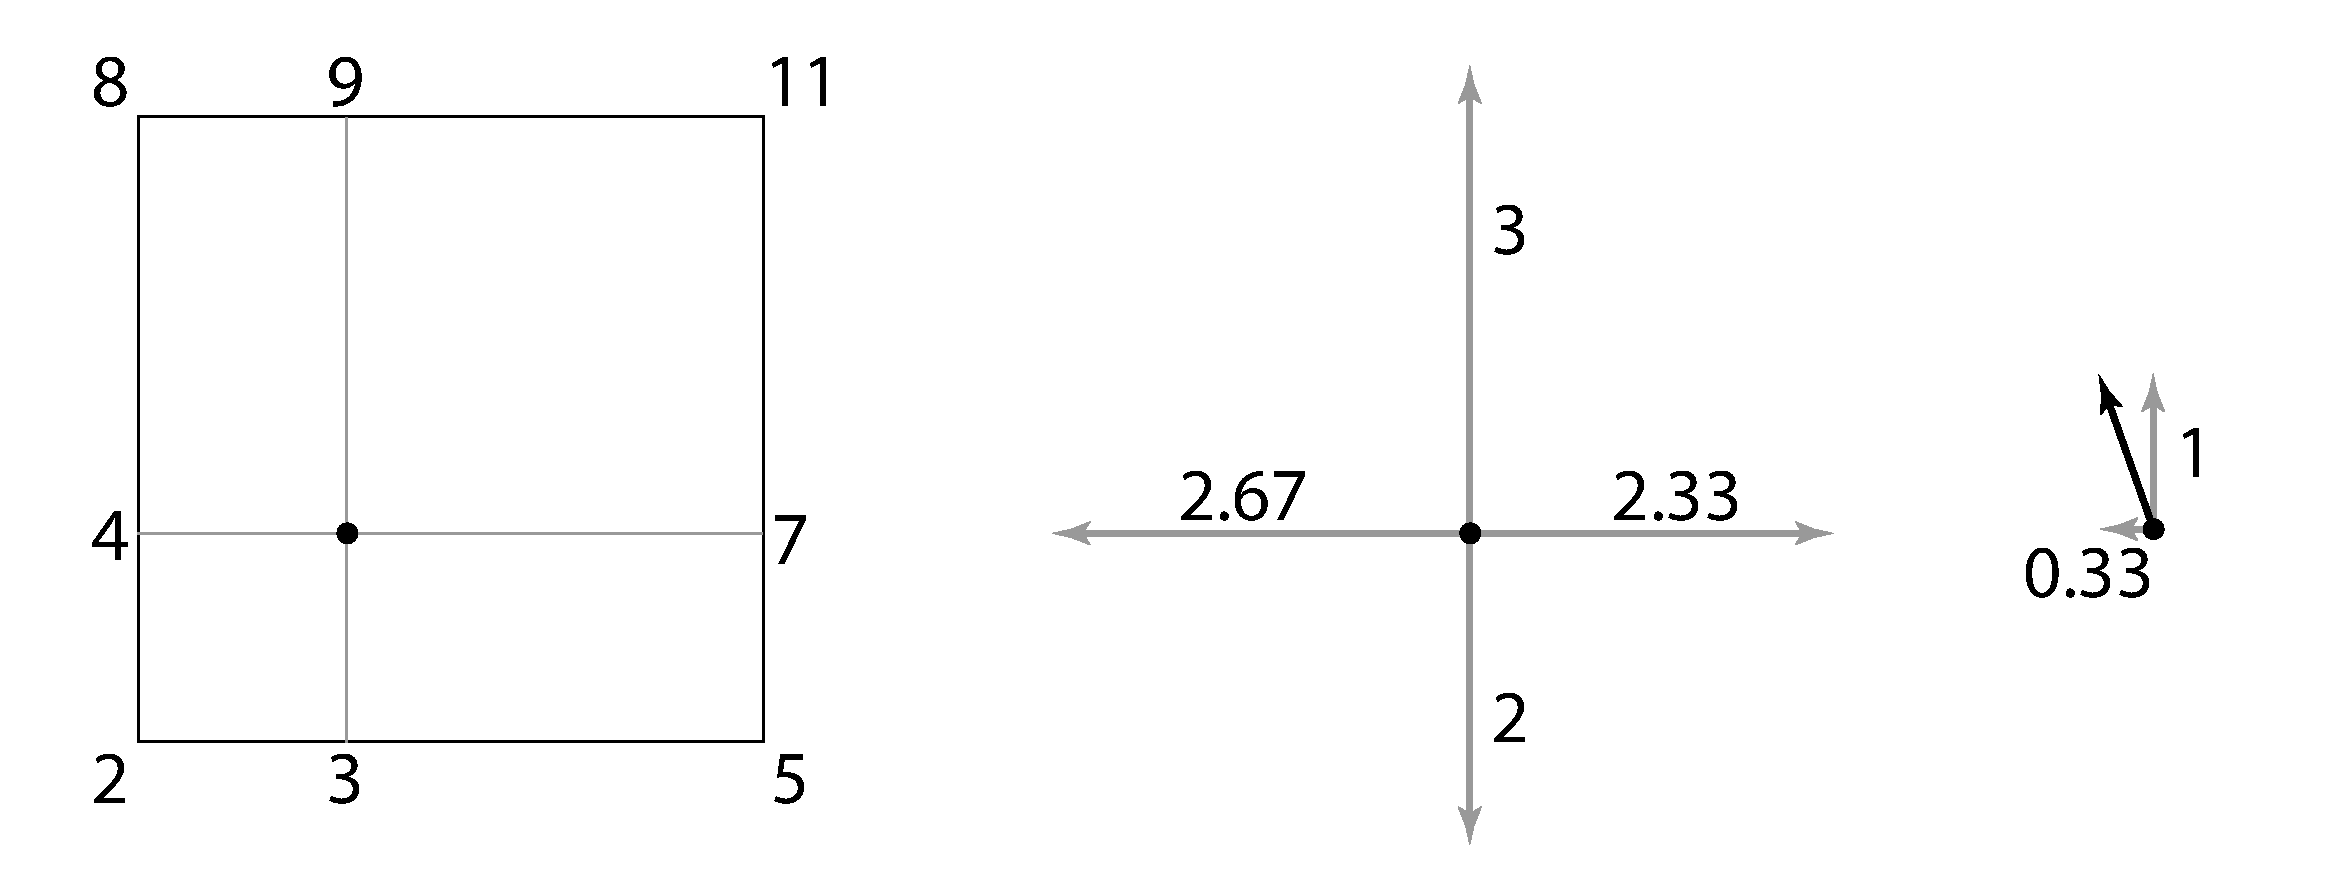
\includegraphics[width=0.8\textwidth]{img/local_gradient_vector.pdf}
    \caption{...}
    \label{fig:vector}
\end{figure}


\subsection{Comparison with Compositing}\label{subsec:opacity_compare}

- Opacity shows volumes, tries to find the edges
- Both show multiple layers
- Opacity clearly shows the structure of the piggy bank (REF), shows the borders of the material
- also the flowers are pretty visible, specially in comparison with composition



\begin{figure}[h!]
    \centering
    \captionsetup{justification=centering,margin=0.5cm}
    \begin{subfigure}[t]{0.49\textwidth}
        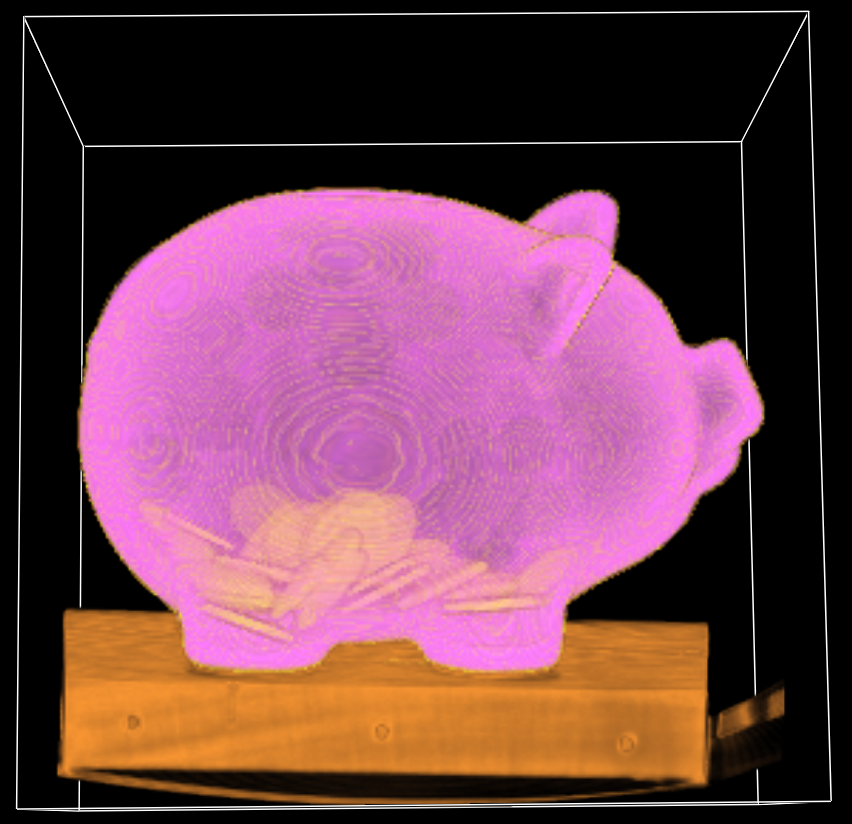
\includegraphics[width=\textwidth]{img/pig-compositing.png}
        \caption{ }
    \end{subfigure}
    \begin{subfigure}[t]{0.49\textwidth}
        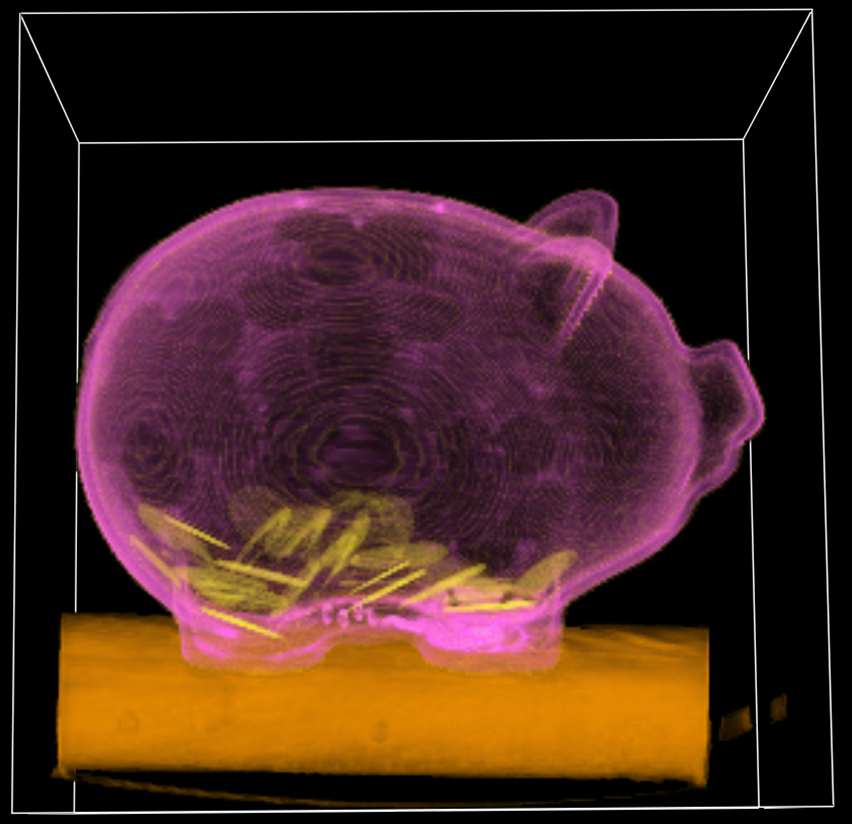
\includegraphics[width=\textwidth]{img/pig-opacity.png}
        \caption{ }
    \end{subfigure}
    \caption{(a) Rendering with compositing raycaster, (b) rendering with opacity weighting raycaster}
    \label{fig:compareraycasters}
\end{figure}


\begin{figure}[h!]
    \centering
    \captionsetup{justification=centering,margin=0.5cm}
    \begin{subfigure}[t]{0.32\textwidth}
        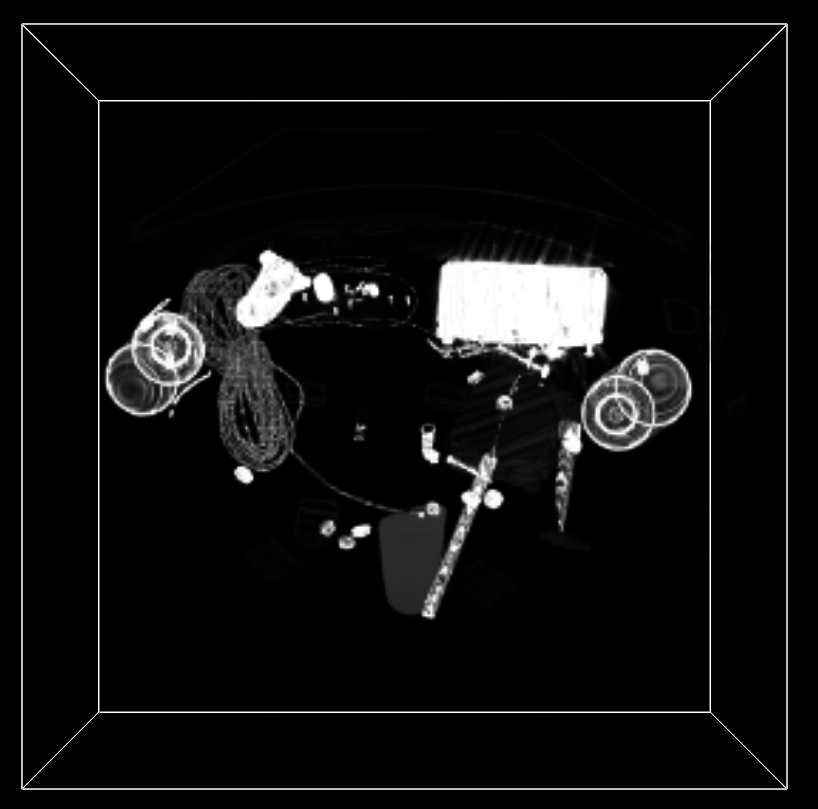
\includegraphics[width=\textwidth]{img/bag-MIP.png}
        \caption{ }
    \end{subfigure}
    \begin{subfigure}[t]{0.32\textwidth}
        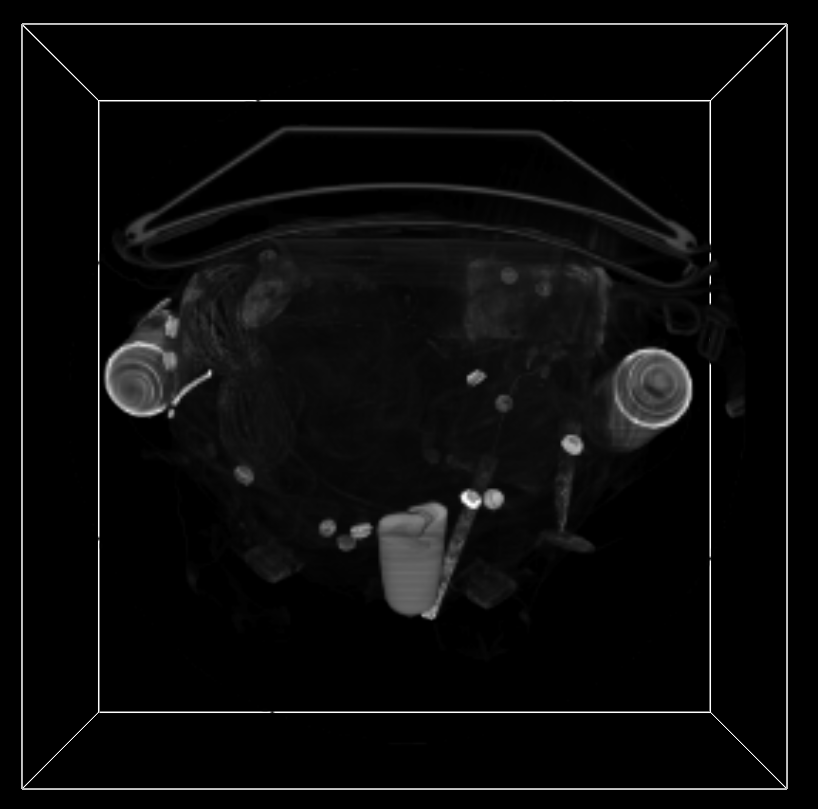
\includegraphics[width=\textwidth]{img/bag-Composition.png}
        \caption{ }
    \end{subfigure}
    \begin{subfigure}[t]{0.32\textwidth}
        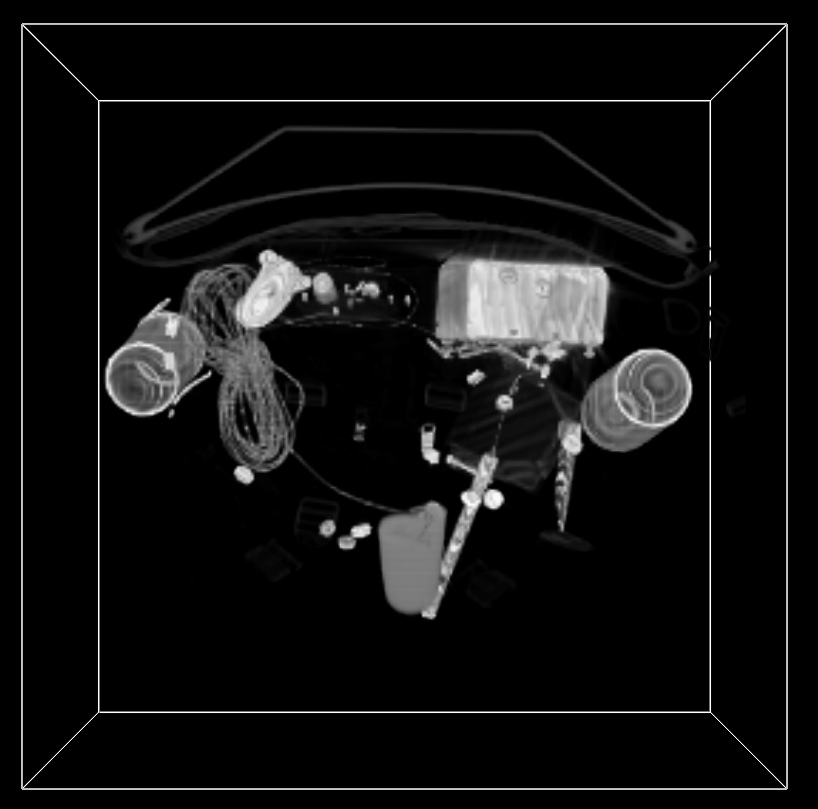
\includegraphics[width=\textwidth]{img/bag-Opacity.png}
        \caption{ }
    \end{subfigure}
    \caption{(a) Rendering with MIP raycaster, (a) Rendering with compositing raycaster, (b) rendering with opacity weighting raycaster}
    \label{fig:compareraycasters}
\end{figure}
